\documentclass{llncs}

\usepackage{llncsdoc}
\usepackage{graphicx,url}
\usepackage[brazil]{babel}
\usepackage[utf8]{inputenc}
\usepackage{float}
\usepackage{setspace}

\usepackage{tabularx}
\usepackage{cite}
\usepackage{hyperref}

\begin{document}
\sloppy
\title{Pushing Together: A platform for social participation}

\author{Tallys Martins\inst{2}, Dylan Guedes\inst{2},
        Luan Guimarães\inst{2}, Paulo Meirelles\inst{1,2}}

\institute{Instituto de Matemática e Estatística -- Universidade de São Paulo (USP)\\
  Rua do Matão, 1010 -- 05508-090 -- Cidade Universitária -- São Paulo -- SP -- Brasil\\
  \email{\{diegoamc,manzo\}@ime.usp.br}
  \and
  Faculdade do Gama -- Universidade de Brasília (UnB)\\
  Gama -- DF -- Brasil\\
  \email{\{tallysmartins,djmgguedes,livreluan\}@gmail.com, paulormm@unb.br}}

\maketitle
\begin{abstract}
  % Contexto
  The brazilian government, as many others around the world, has been trying to
  build technologies for social participation in a collaborative way, exploring
  the guidance of the internet.
  % Problema
  Still, the participation process is more than just giving your opinion, it is
  also about dialog and discussion in a way we should have clear vision about all sides,
  all points of view, all kind of opinions, to discuss what is the best solution
  to a problem. However, the social networks and the recommendation systems, in their
  current design make a barrier in a way that we only receive content about
  what we like, about what we follow, about what our friends like. We are 
  stuck in bubbles of opinion.
  % Soluções propostas
  With this work we present Pushing Together, a free software platform
  for collaborative participation with the aim of breaking the bubbles that
  freezes people in their mindsets. The goal is to identify diferent groups of
  opinion in a conversation using clustering algorithms, and then give power to some
  special actors, bringing interaction between the groups.
  % Frase de impacto
  Through this project we hope to increase the engagement of people in terms of
  social participation and provide new resources for democracy processes.

\textbf{Keywords:} social participation, bubbles of opinion, democracy, gamification
\end{abstract}

\section{Introduction}
\label{sec:intro}
  Promoting social participation is a work made up of many challenges and can be
  analyzed from different aspects. Maybe the biggest one is to discover better
  ways of keeping the process in domain of both, laypeople and empowered ones,
  holding the engagement of the participants.

  Online discussions that happen in the standart ways, such as forums/threads, don’t
  provide an attractive dynamic for those who want to debate. Furthermore, it is
  impractical to do any deeper analysis with the generated information, for example,
  identify what are the opinion groups formed, or yet which opinion is majority
  or minority in discussions that occur in this molds. Natural language processing
  techniques would be extremely difficult to process this kind of information
  given the different themes and contexts of each conversation, outside the
  limitations in working with differents idioms.

  The Pushing Together project applies a different concept for the debates,
  called crowdsourced participation, which has shown to be a great option to break the
  the bariers for engagement and for opening more space to discussions. With little
  effort, the participants can give their opinion from small actions,
  something compared to a simple ‘like’ in a facebook comment.

  Composing people’s opinion in terms of agree and disagree, 0 or 1, it is possible
  to apply clustering algorithms to get sophisticated analysis of what people
  think about a subject in a discussion, and that is where we act.

  Analysing the opinion groups formed, we identify some profiles seen as special actors.
  Applying concepts of gamification we give power for those actors, allowing
  them to interact in the platform creating events and sending direct messages
  to others. With this strategy, we aim to change the communication and expression
  of opinion between different groups, facing what is known as bubbles of opinion,
  created by nowadays digital media.  

  %TODO criar um parágrafo explicando melhor as bolhas

\section{Related tools}

 Existe uma ferramenta que foi construida em cima do conceito de participação
 crowdsourcing e que serviu de inspiração no desenvolvimento do projeto Pushing
 Together. O Polis\footnote{\url{https://pol.is}} oferece aos usuários a possibilidade
 de criar uma discussão em que as pessoas fazem comentários de
 até 140 caracteres demonstrando seu ponto de vista. Os comentários então são
 apresentados como tópicos em cards. A interação na plataforma ocorre com outros
 usuários concordando ou discordando de um comentário existente ou ainda por
 adição de novos comentários à conversa.

 Representando os usuários como um vetores de 0 e 1 para as opções nas propostas
 o Polis aplica um algoritmo de clusterização pateteado e gerando informações
 a respeito dos grupos de opinião formados, propostas mais votadas por grupo, e
 quais propostas foram concordadas ou discordadas pela maioria.

 \begin{figure}[H]
   \centering
   \begin{minipage}{.50\textwidth}
     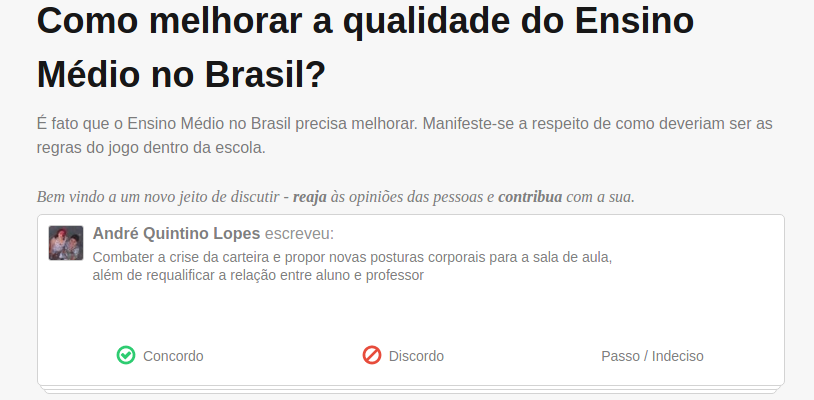
\includegraphics[width=.9\linewidth]{images/polis1.png}
     \caption{Cards with comments}
     \label{fig:polis-2}
   \end{minipage}
   \begin{minipage}{.49\textwidth}
     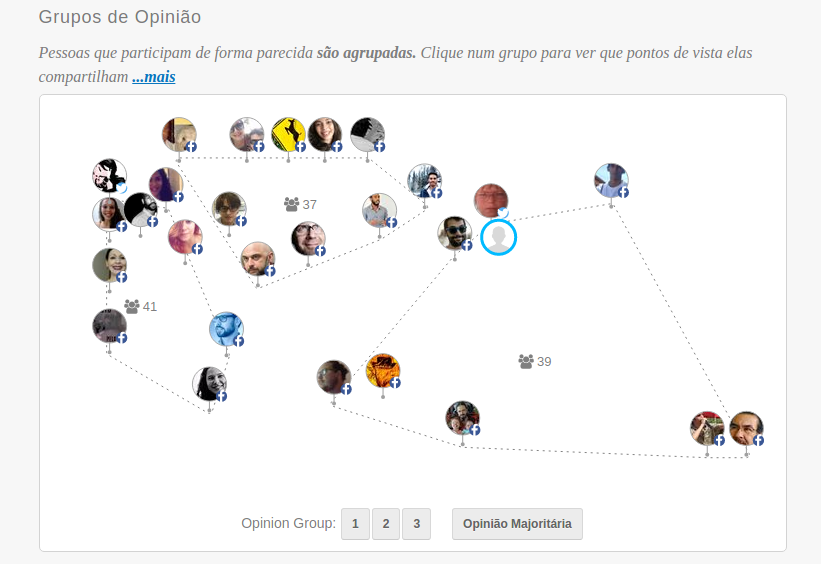
\includegraphics[width=.9\linewidth]{images/polis2.png}
     \caption{Groups of opinion formed}
     \label{fig:polis-1}
   \end{minipage}
 \end{figure}

 Esta ferramenta não contava com os recursos necessários para o desenvolvimento
 do projeto Pushing Together. Era necessário implementar a identificação dos perfis
 chave dentro da clusterização, obter suporte mobile, criar um sistema de notificações,
 entre outros. Assim, a ideia inicial do projeto era contribuir e evoluir a ferramenta Polis
 No entanto, sua comunidade não demonstrou tanta abertura e tivemos dificuldades
 em seguir essa abordagem por falta de documentação, transparência e suporte da
 comunidade criadora do software.

 Com as barreiras encontradas, o projeto nasceu como um sistema arquiteturalmente
 inddependente, encapsulando o Polis em um esforço de engenharia reversa,
 com almejo de uma evolução deste ou, com mais ambição, o desenvolvimento de um serviço próprio
 de clusterização. A segunda opção demonstrou ser mais tangível e foi adotada
 para a continuidade do projeto.

\section{The Pushing Together project}
\label{sec:pushingtogether}

 O Pushing Together nasceu em uma espécie de Hackaton. Uma
 ideia da ONG brasileira Cidades Democráticas que participou do evento chamado Inteligência Coletiva
 para a Democracia, na cidade de Madrid, na Espanha.

 Com o objetivo de facilitar a participação e quebrar as bolhas de opinião,
 o projeto conta com um recurso que chamamos de 'Push', que é parte do conceito
 da gamificação. Os usuários que estiverem em sua posse poderão enviar mensagens
 e criar eventos dentro da plataforma.

 Fazendo uma análise sobre a opinião dos usuários em uma conversa, identificamos
 inicialmente 3 perfis que são considerados os potenciais recebedores do 'Push',

 \begin{figure}[H]
   \centering
     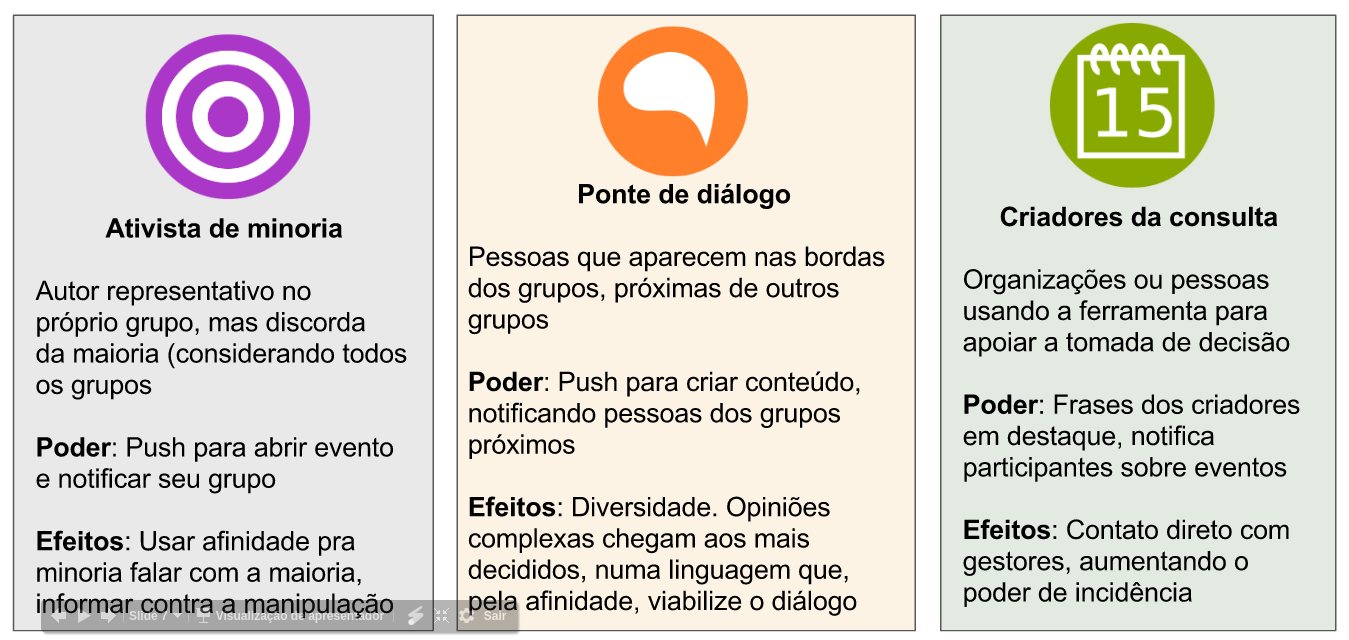
\includegraphics[keepaspectratio=true,scale=0.25]{images/userprofiles.png}
   \caption{User profiles}
   \label{fig:architecture-2}
 \end{figure}

 Com essa modelagem inicial dos perfis espera-se atingir um nível diferenciado
 de interação entre as diferentes opiniões em um grupo de discussão. Essa análise
 dos perfis ainda irá ser testada e validada até sua consolidação.

 Etrando agora em aspectos técnicos, o projeto é dividido em uma
 aplicação front end escrita em React Native e um servidor NodeJS.

 O módulo servidor é responsável por gerenciar os usuários e os
 recursos de push da gamificação, fazendo também a interface com o módulo externo
 de processamento dos clusters. Toda a comunicação, tanto da aplicação front end,
 quanto com o módulo de clusterização é feita através de uma API.
 A figura \ref{fig:architecture-2} abaixo descreve de maneira geral essa arquitetura.

 \begin{figure}[H]
   \centering
     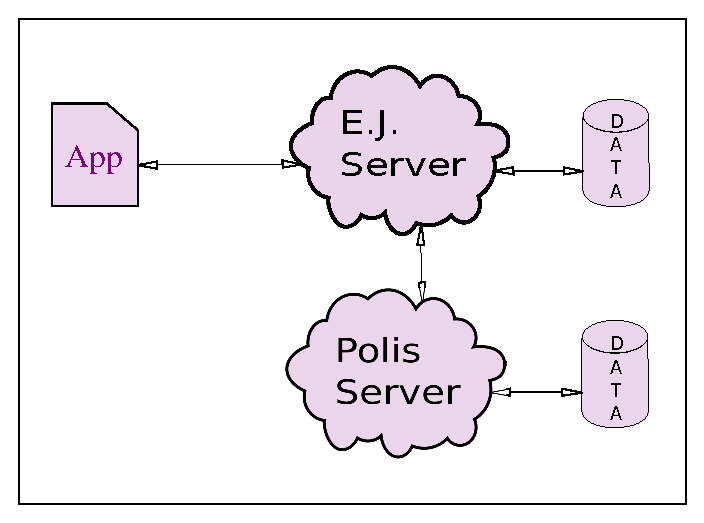
\includegraphics[keepaspectratio=true,,scale=0.5]{images/architecture-1.eps}
   \caption{Architecture of the system}
   \label{fig:architecture-2}
 \end{figure}

\section{Final remarks}

 O Pushing Together surge como uma potencial ponte de diálogo entre a sociedade e o estado,
 fazendo uma análise diferenciada sobre as opiniões dos diferentes grupos, além
 de abrir novas possibilidades para a expressão destas opiniões com o recurso 'Push'.
 E também, o projeto nasce com um princípio de transparência e colarboração,
 para que seja possível a qualquer um se apropriar dos avanços alcançados,
 incentivando a colaboração e consequentemente evoluindo o projeto.

\end{document}
